% Figura cuerpo B1: mapa de las lecturas de la Teoría General y genealogía de las escuelas (temas 3.A.4 a 3.A.7)
\documentclass[tikz,border=3pt]{standalone}
\usepackage[T1]{fontenc}
\usepackage[utf8]{inputenc}
\usetikzlibrary{arrows.meta,calc,positioning}
\begin{document}
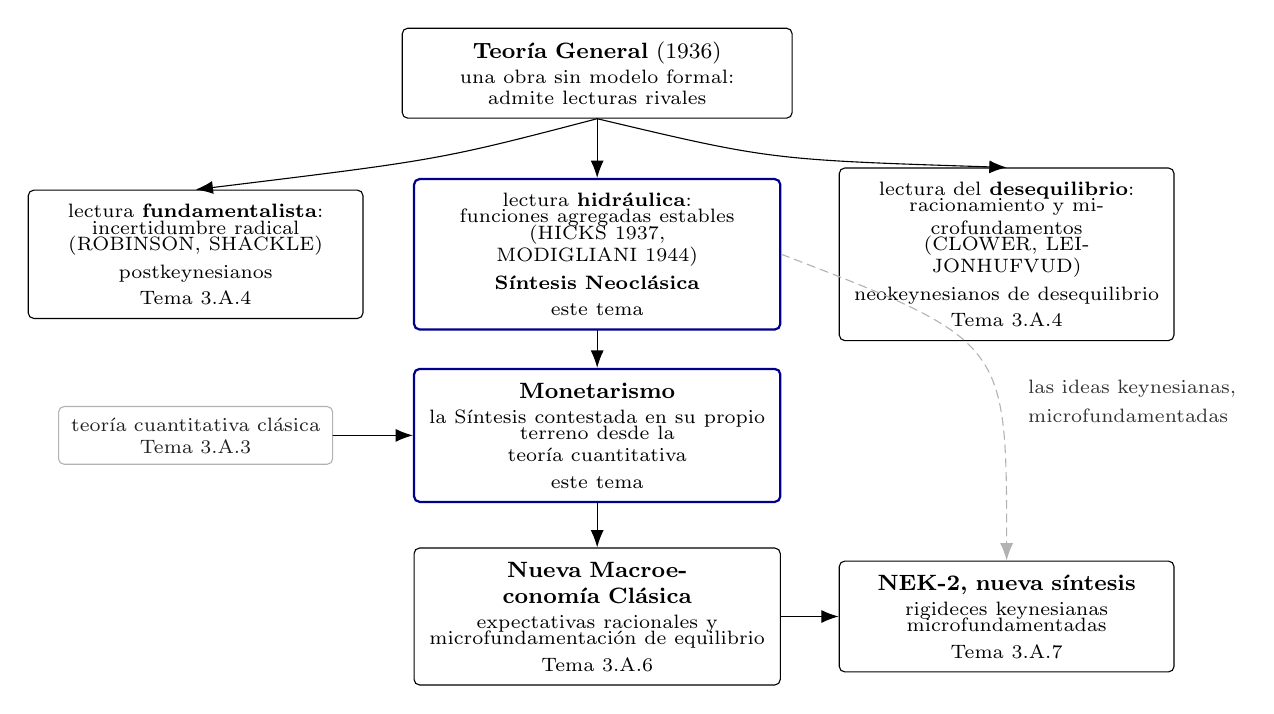
\begin{tikzpicture}[>={Latex[length=2.2mm]}, line cap=round, font=\footnotesize,
  caja/.style={draw, rounded corners=2pt, align=center, inner sep=5pt},
  azul/.style={draw=blue!55!black, thick, rounded corners=2pt, align=center, inner sep=5pt},
  gris/.style={draw=gray!60, rounded corners=2pt, align=center, inner sep=4pt, font=\scriptsize, text=gray!25!black}]
  % Origen
  \node[caja, text width=4.6cm] (tg) at (7.2,6.3) {\textbf{Teoría General} (1936)\\[1pt]\scriptsize una obra sin modelo formal:\\[-2pt]\scriptsize admite lecturas rivales};
  % Tres lecturas
  \node[caja, text width=3.9cm] (fund) at (2.1,4.0) {\scriptsize lectura \textbf{fundamentalista}:\\[-2pt]\scriptsize incertidumbre radical\\[-2pt]\scriptsize (ROBINSON, SHACKLE)\\[2pt]postkeynesianos\\\scriptsize Tema 3.A.4};
  \node[azul, text width=4.3cm] (snc) at (7.2,4.0) {\scriptsize lectura \textbf{hidráulica}:\\[-2pt]\scriptsize funciones agregadas estables\\[-2pt]\scriptsize (HICKS 1937, MODIGLIANI 1944)\\[2pt]\textbf{Síntesis Neoclásica}\\\scriptsize este tema};
  \node[caja, text width=3.9cm] (des) at (12.4,4.0) {\scriptsize lectura del \textbf{desequilibrio}:\\[-2pt]\scriptsize racionamiento y microfundamentos\\[-2pt]\scriptsize (CLOWER, LEIJONHUFVUD)\\[2pt]neokeynesianos de desequilibrio\\\scriptsize Tema 3.A.4};
  \draw[->] (tg.south) ..controls (5.2,5.2).. (fund.north);
  \draw[->] (tg) -- (snc);
  \draw[->] (tg.south) ..controls (9.4,5.2).. (des.north);
  % Monetarismo
  \node[gris, text width=3.2cm] (tcd) at (2.1,1.7) {teoría cuantitativa clásica\\Tema 3.A.3};
  \node[azul, text width=4.3cm] (mon) at (7.2,1.7) {\textbf{Monetarismo}\\[1pt]\scriptsize la Síntesis contestada en su propio\\[-2pt]\scriptsize terreno desde la teoría cuantitativa\\\scriptsize este tema};
  \draw[->] (snc) -- (mon);
  \draw[->] (tcd) -- (mon);
  % Herederos
  \node[caja, text width=4.3cm] (nmc) at (7.2,-0.6) {\textbf{Nueva Macroeconomía Clásica}\\[1pt]\scriptsize expectativas racionales y\\[-2pt]\scriptsize microfundamentación de equilibrio\\\scriptsize Tema 3.A.6};
  \node[caja, text width=3.9cm] (nek) at (12.4,-0.6) {\textbf{NEK-2, nueva síntesis}\\[1pt]\scriptsize rigideces keynesianas\\[-2pt]\scriptsize microfundamentadas\\\scriptsize Tema 3.A.7};
  \draw[->] (mon) -- (nmc);
  \draw[->] (nmc) -- (nek);
  \draw[->, densely dashed, gray!60] (snc.east) ..controls (12.4,2.9).. (nek.north);
  \node[gray!40!black, font=\scriptsize, anchor=west] at (12.55,2.3) {\scriptsize las ideas keynesianas,};
  \node[gray!40!black, font=\scriptsize, anchor=west] at (12.55,1.95) {\scriptsize microfundamentadas};
\end{tikzpicture}
\end{document}
